% !TeX document-id = {a90a2b0a-e08e-44ed-850a-35793bedbf3a}
% !TeX TS-program = xelatex

% !BIB program = biber
\documentclass[handout]{beamer}
%\documentclass[compress]{beamer}
\usepackage[T1]{fontenc}
\usepackage{pifont}
\usetheme[block=fill,subsectionpage=progressbar,sectionpage=progressbar]{metropolis} 


\definecolor{Purple}{HTML}{911146}
\definecolor{Orange}{HTML}{CF4A30}

% Theme colors are derived from these two elements
\setbeamercolor{alerted text}{fg=Orange}

% ... however you can of course override styles of all elements
\setbeamercolor{frametitle}{bg=Purple}


\usepackage{wasysym}
\usepackage{etoolbox}
\usepackage[utf8]{inputenc}

\usepackage{threeparttable}
\usepackage{subcaption}

\usepackage{tikz-qtree}
\setbeamercovered{still covered={\opaqueness<1->{5}},again covered={\opaqueness<1->{100}}}


\usepackage{listings}

\lstset{
	basicstyle=\scriptsize\ttfamily,
	columns=flexible,
	breaklines=true,
	numbers=left,
	%stepsize=1,
	numberstyle=\tiny,
	backgroundcolor=\color[rgb]{0.85,0.90,1}
}



\lstnewenvironment{lstlistingoutput}{\lstset{basicstyle=\footnotesize\ttfamily,
		columns=flexible,
		breaklines=true,
		numbers=left,
		%stepsize=1,
		numberstyle=\tiny,
		backgroundcolor=\color[rgb]{.7,.7,.7}}}{}


\lstnewenvironment{lstlistingoutputtiny}{\lstset{basicstyle=\tiny\ttfamily,
		columns=flexible,
		breaklines=true,
		numbers=left,
		%stepsize=1,
		numberstyle=\tiny,
		backgroundcolor=\color[rgb]{.7,.7,.7}}}{}


\usepackage[american]{babel}
\usepackage{csquotes}
\usepackage[style=apa, backend = biber]{biblatex}
\DeclareLanguageMapping{american}{american-UoN}
\addbibresource{../literature.bib}
\renewcommand*{\bibfont}{\tiny}

\usepackage{tikz}
\usetikzlibrary{shapes,arrows,matrix}
\usepackage{multicol}

\usepackage{subcaption}

\usepackage{booktabs}
\usepackage{graphicx}

\graphicspath{{../pictures/}}

\makeatletter
\setbeamertemplate{headline}{%
	\begin{beamercolorbox}[colsep=1.5pt]{upper separation line head}
	\end{beamercolorbox}
	\begin{beamercolorbox}{section in head/foot}
		\vskip2pt\insertnavigation{\paperwidth}\vskip2pt
	\end{beamercolorbox}%
	\begin{beamercolorbox}[colsep=1.5pt]{lower separation line head}
	\end{beamercolorbox}
}
\makeatother



\setbeamercolor{section in head/foot}{fg=normal text.bg, bg=structure.fg}



\newcommand{\question}[1]{
	\begin{frame}[plain]
		\begin{columns}
			\column{.3\textwidth}
			\makebox[\columnwidth]{
				
\includegraphics[width=\columnwidth,height=\paperheight,keepaspectratio]{../pictures/mannetje.png}}
			\column{.7\textwidth}
			\large
			\textcolor{orange}{\textbf{\emph{#1}}}
		\end{columns}
\end{frame}}

\newcommand{\instruction}[1]{\emph{\textcolor{gray}{[#1]}}}


\title[Computational Communication Science 2]{\textbf{Computational Communication Science 2} \\Week 8 - Lecture\\ »A Deep Dive into Supervised Machine Learning«}
\author[Marthe Möller, Anne Kroon]{Marthe Möller \\ Anne Kroon \\ ~ \\ \footnotesize{a.m.moller@uva.nl, @marthemoller \\a.c.kroon@uva.nl, @annekroon} \\}
\date{May, 2022}
\institute[Digital Society Minor, University of Amsterdam]{Digital Society Minor, University of Amsterdam}


\begin{document}
	
	\begin{frame}{}
		\titlepage
\end{frame}
	
\begin{frame}{Today}
		\tableofcontents
\end{frame}


\section{Recap}

\begin{frame}{Recap}
	
Last week, we talked about:
	\begin{itemize}
		\item Rule-based Text Classification
		\item Automated Text Classification: SML
		\item The principles behind SML
		\item The steps of SML
		\item Some commonly used ML models
		\item Validating models \\\
	\end{itemize}
	
At home, you:
	\begin{itemize}
		\item Worked with SML (homework assignment)
	\end{itemize}
	
\end{frame}


\begin{frame}{Recap}
	
Today, we:
	\begin{itemize}
		\item Talk about the homework that you did
		\item Take a deep dive in SML
		\item Take a critical look at SML 
	\end{itemize}
	
\end{frame}


\section{SML in practice}


\begin{frame}{Cross-validation}
	
Let's review the homework assignment!
	
\end{frame}



\begin{frame}{Neural Networks}
	
	\begin{center}
		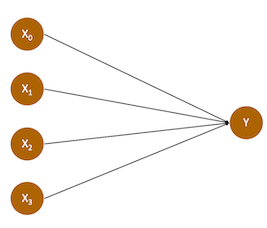
\includegraphics{../pictures/perceptron.png} \\\
	\end{center}
	
	% What does a computer actually do with the models discussed above? In this lecture, we discuss neural networks as a machine learning algorithm.
	
	% Neural networks consist of connection between neurons that are activated if the total input is above a certain threshold. Simplest form: perceptron.
	
	% A perceptron is a single-layer neural network.
	
	% Input neurons (or IV’s) connected to an output neuron (or DV). Each of the connections between neurons has a weight which can be positive or negative. For the output neuron, the weighted sum of inputs is calculated and a function is applied to determine the results. Which function is not set, it could be, for example, a logistic regression!
	
\end{frame}


\begin{frame}{Neural Networks}
	
	\begin{center}
		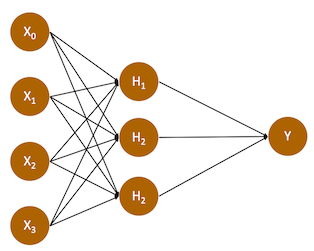
\includegraphics{../pictures/neuralnetwork_hiddenlayer.png} \\\
	\end{center}
	
	\begin{tiny}
		\fullcite{ha_automatically_2021} 
	\end{tiny}
	
	% Imagine we use machine learning to determine the positivity or negativity of online movie reviews (sentiment analysis). The input neurons could be the frequencies of words such as “great” (positive weight) and “horrible” (negative weight). Such a network is a bit simplistic, because a review that says something is “not great” is negative but this wouldn’t be picked up by our network.
	
	% To solve this, we can add a hidden layer of latent variables between the input and the output layer of the network.
	
	% Connect to Ha et al. (link to deep learning)
	
	
\end{frame}




\section{Cross-validation}

\begin{frame}{Cross-validation}

We talked about validating models.

\end{frame}



\begin{frame}{Cross-validation}
	
	Overfitting: When a model fits \emph{exactly} against the data.
	
	When we calculate the metrics discussed above for multiple models on the same test dataset, we run the risk of overfitting on the test data.
	
	Potential solution: Split the dataset into three smaller sets. A training dataset, a validation dataset and a test dataset.
	
	However, this requires us to have a very large labeled dataset. In reality, this is not always the case!
	
	%Consequence of this is, for example, that your model can classify your training data perfectly, but it can't classify other data very well anymore.
	
	%Overfitting the model generally takes the form of making an overly complex model to explain idiosyncrasies in the data under study. In reality, the data often studied has some degree of error or random noise within it. Thus, attempting to make the model conform too closely to slightly inaccurate data can infect the model with substantial errors and reduce its predictive power.
	
\end{frame}


\begin{frame}{Cross-validation}
	
	Cross-validation: A resampling procedure to evaluate ML models on a limited data sample.
	
	\(k\)-fold cross-validation, where \(k\) refers to the number of groups or folds in which a sample is split.

\end{frame}


\begin{frame}{\(k\)-fold cross-validation}
	\(k\)-fold cross-validation step by step:
	\begin{enumerate}
		\item Shuffle the data
		\item Split the data into \(k\) folds (groups)
		\item For each unique group
		\begin{enumerate}
			\item Take the group as a test dataset
			\item Take the remaining groups as one training dataset
			\item Fit a model on the training set and evaluate it on the test set
			\item Retain the evaluation score and discard the model
		\end{enumerate}
		\item Summarize the evaluation scores to assess the model \\\
	\end{enumerate}

\end{frame}
	

\begin{frame}{Cross-validation}
	
	Cross-validation is often used to compare many different model specifications, for example to find the best hyperparameters.
	
	Hyperparameters: Parameters of the model that are not estimated from the data. 
	
	To do this, the Grid Search algorithm is often used.
	
	More about hyperparameters in this week's tutorial!
	
\end{frame}




\begin{frame}{Zooming out} 
	
	We talked about:
	\begin{itemize}
		\item SML in practice
		\item Cross-validation \\\
	\end{itemize}
	
	Next, we will talk about:
	\begin{itemize}
		\item Strengths and challenges associated to SML
	\end{itemize}
	
\end{frame}


\section{SML: Strenghts and Challenges}


\begin{frame}{Strengths and Challenges} 
	
	Strengths:
	\begin{itemize}
		\item Easier to code large datasets
		\item Enhances replicable research
		\item Easier to study "natural" human behavior \\\
	\end{itemize}
	
	Disadvantages:
	\begin{itemize}
		\item Resource constraints
		\item Ethical considerations
		\item Criticism required (see next slide)
	\end{itemize}

% Strengths:
% -	Makes it easier to code large datasets (cheaper, faster)
% -	Enhances replicable research (exactly the same script can be used to by researchers to conduct a new content analysis)
% -	Makes it easier to study “natural” human behavior (example: study social influence by hiring actors to see if it influences people’s reactions to videos; now, we can just analyze the comments people write and how these influence subsequent comments!)

% Challenges
% -	(Jordan & Mitchell, p. 5) Resource constraint (privacy, required processing capacities  communication constraint
% -	Ethical questions: Who will have access to, and ownership of, online data and who will reap its benefits? (Jordan & Mitchell, p.6)

\end{frame}


\begin{frame}{Strengths and Challenges}
	
	\begin{center}
		
\includegraphics[width=\linewidth,height=\textheight,keepaspectratio]{../pictures/toeslagenaffaire_headlines.png} \\\
	\end{center}
	
% As shown by Jordan & Mitchell, ML is used in many different facets of society. But it is impertinent that those who use ML remain critical of its capabilities. If a machine is trained based on human coded data, as is the case with SML, it will also learn about the prejudices that humans have: toeslagenaffaire voorbeeld. Laag inkomen werd door computer geleerd als voorspeller van fraude. Mensen met een laag inkomen werden er dus bij voorbaat al uitgepikt. 
%  Remember that in the end, machines are created by humans and as humans we are responsible for how we use them. We have the responsibility to ask questions about what machines do and how and whether we should!
	
\end{frame}


\begin{frame}{Zooming out} 
	
	We talked about:
	\begin{itemize}
		\item SML in practice
		\item Cross-validation
		\item Strengths and challenges associated to SML \\\
\end{itemize}
	
This week's tutorial:
	\begin{itemize}
		\item Hands-on approach to take a further look into the machine learning process
		\item Tutorial goal:
		\begin{itemize}
			\item To provide a stepping stone so that you can (independently) advance your machine learning skills
		\end{itemize}
		
	\end{itemize}
	
\end{frame}


\end{document}